\chapter{Introduction}
The robot-assisted system for endodontic treatment is presented in this thesis. The definition of a robot-assisted system in the present thesis refers to be a dental assistant. 
We have studied some related dental robot. There are brief introductions of the endodontic treatment, previous work ,and the proposed method in this chapter.
\section{Motivation}
\hspace*{6mm}The performance of the endodontic treatment depends on the dentist's long-term expertise. A qualified dentist can operate the endodontic treatment and accumulate their experience to increase the success rate. With many experiences, dentists can acquire an endodontist license. According to statistics from the Ministry of Health and Welfare, R.O.C. (Taiwan) \cite{web1}, the number of dentists in Taiwan is $15,178$. However, according to The Academy of Endodontology, R.O.C. (Taiwan) \cite{web2}, there are only $238$ dentists to acquire an endodontist license due to the expertise of endodontics. 
\par
Besides, Root canal treatment is tedious and time-consuming due to the complicated conditions of each tooth. A patient who suffered from an infected tooth spends countless hours see a dentist. It takes at least two to three rounds, even takes more than two months in the worst case. 
\par
Therefore, our team looks forward to designing a robot-assisted system to finish the root canal treatment.  With the system, we wish it can increase the success rate of the root canal treatment for dentists and provide patients a safe surgery.
\section{Previous Work and Problem Definition}
\hspace*{6mm}First, we introduce the endodontic treatment and its detailed procedure.
\par
Endodontic treatment, also known as root canal treatment and nerve extraction, is performed to cure an infected tooth. The procedure of endodontic treatment is divided into three parts - Opening, Cleaning, and Filling shown in  Figure \ref{fig:endo-procedure}.
\begin{figure}[htbp]
\begin{center}
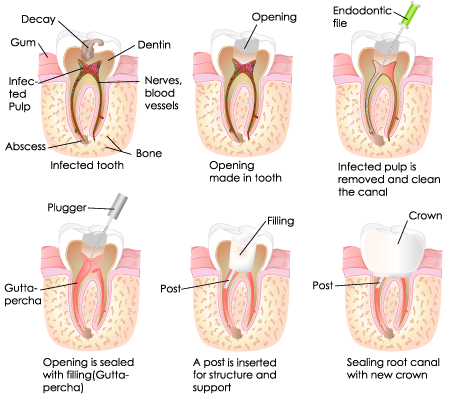
\includegraphics[width=0.8\linewidth]{Images/endo-procedure.png}
\caption{
The endodontic therapy steps
}\label{fig:endo-procedure}
\end{center}
\end{figure}
\par
An infected tooth arises from periodontal disease, attrition, trauma, or decay. Once the dental pulp is infected, it causes an irreversible inflammation and lets patients confront a root canal treatment. Figure \ref{fig:endo-procedure} shows an infected tooth and its dental pulp, which consisted of blood vessels, nerves, connective tissues, and lymphatics. In the "Opening" step, an experienced dentist drills the crown of the infected tooth to remove the dentin and expose the infected pulp inside the canal to the air. Next, in the "Cleaning" step, the dentist uses an endodontic file, a flexible reamer, to remove the infected pulp. Then, in the "Filling" step, the dentist uses a dental plugger to fill the empty root canal with Gutta-percha, a plastic substance. "Filling" can prevent cross-infection between root canals because the cured tooth remains many invisible and inaccessible pulp tissue. Finally, the dentist seals the root canal with a new crown to protect cured root canal. 
\par
As stated above, "Cleaning" is of paramount importance in a whole treatment because untreated cleaning will result in pulp necrosis, apical abscess, periodontal ligament inflammation, or even cellulitis. If there are many remained infected pulp after root canal treatment, the surgery should be operated on again. "Cleaning" procedure is a big challenge in and of itself. Therefore, we should figure out how to enable the robot to assist dentists and perform the root canal treatment.
\par
There are more and more robots which applied to specific surgery. In the dental field, the majority of robotic applications are in implant surgery. The researchers in Chosun University built a dental implant robot \cite{Kim2009ASO}, which is a remote center of motion (RCM) mechanism. Li, J.et al built a robotic system using soft bracing technique to drill teeth \cite{Li2019ACD}. Also, there is the first commercial implant robot, YOMI, developed by Neosis \cite{web3}. YOMI has received the clearance from FDA and has performed more than $2,700$ times surgery in the USA. In the pandemic of Covid-19 in 2020, YOMI provided non-contact surgery between dentists and patients due to its automatic robotic system. However, there was one and only one robot for the endodontic treatment. The domestic researcher Janet Dong and his team designed a draft of an endodontic micro robot. They proposed a micro robot performing root canal treatment with the assistance of a 3D computer model system. It is designed to accomplish endodontic therapy with a path planned according to the 3D model. Whereas, the study using 3D model is belongs to pre-operation. If there is a movement caused by patients or image error, it will not easy to reschedule the motion planning because the root canal in a tooth is unseen by any camera. Besides, once a root reamer enters into a root canal, it is hard to obtain the position of the tool tip due to its flexibility. The root reamer will bend when it bears a force. Once we lose the position of the endodontic file, it may lead to perforation, overpreparation, and inderpreparation. Therefore, there is a problem remains - how the robot know the path of a root canal without visual feedback?   
\par
On the other hand, instrument fracture is the concern during the therapy. If the endodontic file suffered excessive usage, it would unpredictably break. The leading causes of fractured files are torsional fracture and flexural fatigue, which account for 55.7\% and 44.3\% separately \cite{SATTAPAN2000161}. Removal of broken files is technically difficult, so it is essential to reduce the probability of the instrument fracture. Therefore, our robot should prevent the instrument fracture by some detection. In addition, the root canal treatment also requires repeatedly drilling to clean the canal thoroughly and a motion planning to prevent perforation. This repetitive action of root canal treatment is tedious and time-consuming. Therefore, we decide to design an automatic endodontic robot to improve the time efficiency and prevent instrument fracture in endodontic surgery.	
\par\noindent
In sum up, what problems the thesis encounter are 
\begin{enumerate}
\item How to assist dentists to perform the root canal treatment including motion planning, especially in the second procedure - cleaning?
\item How to overcome the problem that the root canal cannot be visually observed, and how to clean well in any complex conditions?
\item How to protect the endodontic file from fracturing during the surgery?
\end{enumerate}	
\section{The Proposed Method}
(Solutions: (be consistent with problem definition)
1.	Build a robot-assisted system and enable it to drill
2.	Force-guided alignment 
3.	Control the file rotation speed
we use current feedback to keep track of the file's torque during the endodontic treatment.
B.	Prospect:
\par\noindent
(Prospect: Move to the infected teeth$\longrightarrow $Root canal searching$\longrightarrow $Repetitive drilling$\longrightarrow $Apex Detection)						
\section{Main Contributions of the Thesis}
\begin{enumerate}
	\item	Integrate a 6-DoF robotic manipulator with 6-DoF F/T sensor for performing endodontic treatment.
	\item	Develop a framework for robot alignment regarding the position and orientation of root canal. 
	\item	Protect the endodontic file from fracturing by controlling file rotation speed.
\end{enumerate}
\section{Organization of the Thesis}
\hspace*{6mm}The structure of this thesis is as follows.